\documentclass[a4paper,11pt,exos]{nsi} % COMPILE WITH DRAFT
\usepackage{pifont}
\usepackage{fontawesome5}
\usepackage{hyperref}



\begin{document}
\classe{\terminale Comp}
\titre{Modèles utilisant le logarithme}
\maketitle

\subsection*{Intensité et niveau sonore}
La fonction logarithme décimal est définie sur $\oio{0}{+\infty}$ par $\log(x)=\dfrac{\ln(x)}{\ln(10)}$.\\
Elle vérifie les mêmes propriétés algébriques que la fonction logarithme népérien.\\
En physique, le \textbf{niveau sonore} $N$ en décibels (dB) d'un son d'un son d'\textbf{intensité acoustique} $I$ en watt par m$^2$ est donné par la relation $N(I)=10\log\left(\dfrac{I}{I_0}\right)$ où $I_0=10^{-12}$ W/m$^2$ est la plus faible intensité perceptible par l'oreille humaine.

\subsubsection*{Partie A : Quelques exemples}
\dleft{9cm}{
    \begin{enumerate}
        \item Quel est le niveau sonore $N_0$ d'un son d'intensité acoustique $I_0$ ?
        \item L'intensité acoustique d'une moto est estimée à $10^{-5}$ W/m$^2$.\\
        Quel est le niveau sonore de cette moto ?
        \item Le niveau sonore d'une salle de classe est estimé à 60 dB.\\
        Quelle est l'intensité acoustique de cette salle ?
        \item Les scientifiques estiment que le seuil de douleur est atteint à partir d'un niveau sonore de 120 dB.\\
        Quelle est l'intensité acoustique correspondante ?
    \end{enumerate}
}
{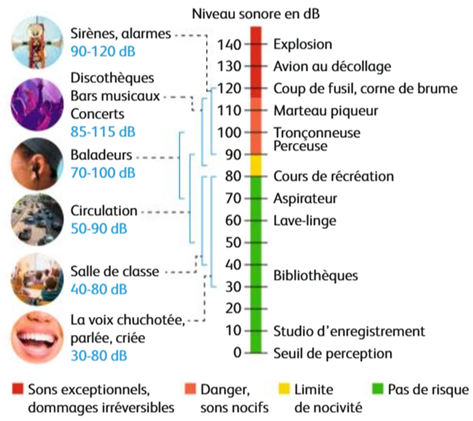
\includegraphics[width=7.5cm]{niveaux_sonores.png}}

\vspace*{.5cm}
\dleft{10.5cm}{
    \subsubsection*{Rapport entre niveau sonore et intensité acoustique}
    \begin{enumerate}
        \item L'intensité de la sonnerie d'un téléphone portable est de 60 dB, celle d'un avion au décollage à 200 m est 120 dB.\\
        Combien faudrait-il de téléphones portables pour atteindre le niveau sonore d'un avion au décollage à 200 m ?
        \item \textbf{Vrai ou faux ?} : Si l'intensité acoustique est multipliée par 10, le niveau sonore augmente de 10 dB.
        \item Le 9 août 2017, la législation sur le niveau sonore dans les discothèques et les salles de concert a évolué. Le niveau sonore moyen, mesuré sur 15 minutes, ne peut plus dépasser 102 décibels, alors que le niveau maximal était fixé à 105 décibels depuis 1998.\\
        Comment a évolué l'intensité acoustique maximale autorisée ?
    \end{enumerate}
}
{
    \small\textbf{Durée limite d'exposition (sans protection) avant dommage auditif} :
    \begin{enumerate}[label=\textbullet]
        \item De 120 à 140 dB : quelques secondes suffisent à provoquer des lésions irréversibles ;
        \item 100 dB : 5 min par jour ;
        \item 95 dB : 15 min par jour ;
        \item 92 dB : 30 min par jour ;
        \item 89 dB : 1 h par jour ;
        \item 86 dB : 2 h par jour ;
        \item 80 dB : 8 h par jour.
    \end{enumerate}
}

\subsection*{Sismologie}
\dleft{14.2cm}{
    \begin{encadrecolore}{Info :}{UGLiDarkBlue}
        \small Deux paramètres sont utilisés pour mesurer la force des séismes : la \textbf{magnitude} et l'\textbf{intensité}.\\
        Un séisme est associé à une seule \textbf{magnitude} et à une gamme de valeurs d'\textbf{intensité}. En effet, la magnitude caractérise l'énergie libérée par la rupture de la faille à l'origine des secousses tandis que l'intensité sismique varie d'un site à l'autre pour un même séisme (par exemple : ressenti des habitants, dégâts matériels, etc.).\\
        Les médias font souvent référence à la \textit{magnitude du séisme sur l'échelle ouverte de Richter}. Elle a été définie en 1935 par Charles Francis Richter qui a établi une échelle pour classer et comparer les séismes californiens.
    \end{encadrecolore}
}
{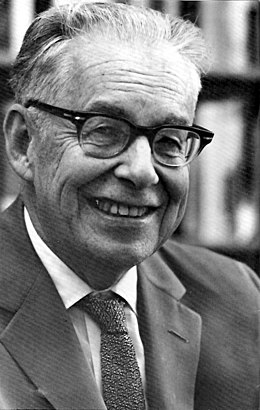
\includegraphics[width=2.2cm]{CharlesRichter.jpg}\\
\tiny{Charles Francis Richter vers 1970}}

\subsubsection*{Magnitude d'un séisme}
L'échelle de Richter, basée sur les mesures faites par les sismographes, exprime la magniture $M$ d'un séisme.\\
Cette magnitude est définie par la relation $M=\log\left(\dfrac{A}{A_0}\right)$ où $A$ est l'amplitude maximale relevée par le sismographe et $A_0$ est une amplitude de référence ; $\log$ est la fonction logarithme décimal définie sur l'intervalle $\oio{0}{+\infty}$ par $\log(x)=\dfrac{\ln(x)}{\ln(10)}$.
\begin{enumerate}
    \item Que vaut la magnitude d'un séisme si l'amplitude relevée est 10 000 fois plus grande que l'amplitude de référence ?
    \item Un séisme est dit « léger » si sa magnitude est comprise entre 4 et 5.\\
    Monter que son amplitude $A$ vérifie alors $\quad 10^4 \times A_0\leqslant 
    A\leqslant 10^5\times A_0$.
    \item La magnitude connue la plus importante est de 9,5. Elle a été enregistrée lors du séisme de Valdivia au Chili en 1960. Démontrer que son amplitude $A$ vérifie $\quad A=\sqrt{10}\times 10^9 A_0$.
    \item Un pays vient de connaître un séisme de magnitude 8 suivi d'une réplique de magnitude 4. Un journaliste écrit alors que la réplique a été deux fois moins puissante que le premier séisme.\\
    Qu'en pensez-vous ?
\end{enumerate}

\subsubsection*{Énergie libérée par un séisme}
L'énergie $E$, en joule (J), libérée par un séisme se calcule à l'aide de l'égalité $\quad \log(E)=a+bM$\\
où $M$ est la magnitude du séisme et $a$ et $b$ sont deux nombres réels.\\
Plus le séisme a libéré d'énergie, plus sa magnitude est élevée.\\
Un accroissement de 1 de la magnitude correspond à une multiplication par 30 de l'énergie libérée.
\begin{enumerate}
    \item Justifier que $a$ et $b$ sont solutions du système $(S)$ :
     $\left\{
			\begin{array}{l}
				\ \log(E)=a+bM \\
				\ \log(30E)=a+b+bM \\
			\end{array} \right.$
    \item Déterminer $a$ et $b$ sachant qu'un séisme de magnitude 3 a libéré une énergie égale à $6,4\times 10^{15}$ joules. \textit{Arrondir au centième}.
    \item Calculer l'énergie libérée au foyer d'un séisme de magnitude 5.
\end{enumerate}

\newpage
\end{document}